Durante fase di progettazione di applicazioni come Mole.io, non si pu� prescindere dal prendere in considerazione il carico di lavoro che subir� il sistema in produzione ed i tempi di risposta attesi. 

Le tecniche di ottimizzazione del Database e di sharding dei dati, da sole, non bastano a garantire buone performance del sistema. \`{E} necessaria, infatti, una organizzazione dell'architettura del sistema che renda performanti le diverse operazioni verso il Database e, nello stesso tempo, non limiti le possibilit� di estensione futura del sistema stesso.

Il \textit{Command Query Separation} (CQS) � un principio di programmazione, discusso da  Bertrand Meyer in \cite{meyer1988object-oriented}. Dichiara che, in un sistema software, ogni metodo deve appartenere ad una sola delle seguenti categorie:
\begin{description}
\item[Command] un metodo che esegue azioni, modifica i dati, non restituisce alcun risultato e crea potenzialmente \textit{inconsistenza} nel sistema; 
\item[Query] un metodo che ottiene dati esistenti, esegue richieste e restituisce risultati senza alterare lo stato del sistema;
\end{description}

La descrizione del principio in una sola frase potrebbe essere: \textit{porre una domanda non dovrebbe cambiare la risposta}.

Nonostante il CQS sembri un concetto molto semplice, la sua implementazione all'interno dei sistemi � tutt'altro che immediata. Il principio, infatti, � inteso come linea guida e come invito alla separazione netta delle competenze di ogni funzione o modulo.

Il \textit{Command Query Responsibility Segregation} (CQRS) � un pattern architetturale che segue le regole indicate dal CQS e le applica al design di sistemi software. L'idea alla base di questo pattern, infatti, � la separazione netta dei moduli di scrittura (command) e lettura (query) presenti in una applicazione. Spesso la separazione si estende al database stesso, ottenendo cos� sistemi con due basi di dati: una utilizzata esclusivamente per eseguire scritture e l'altra per eseguire letture.

I sistemi CQRS sono disegnati in modo da separare le responsabilit� di scrittura e lettura. Questo approccio solleva immediatamente un problema, come � possibile scrivere dati all'interno di un database e pretendere di leggerli da un archivio differente? La risposta risiede nei \textit{denormalizzatori}.

Un denormalizzatore � un modulo software che ha il compito di creare duplicazione di informazione. Esso, infatti, legge dati salvati in formato grezzo e li elabora, ristrutturandoli, per fare in modo che essi diventino facilmente fruibili per la lettura. A questo punto li salva nuovamente all'interno del database. Nel caso di sistemi con due database, i denormalizzatori sono gli unici attori nel sistema che leggono dati dal database di scrittura e li scrivono nel database di lettura.  

Il principale vantaggio offerto da CQRS � la possibilit� di ottimizzare separatamente i database di lettura e scrittura. Ad esempio, la presenza di \textit{indici} sulle tabelle di lettura, velocizza molto le operazioni di recupero dei dati, mentre penalizza quelle di scrittura, a causa della necessit� di aggiornamento degli indici a fronte di un inserimento. La separazione delle tabelle di lettura e scrittura permette di attivare gli indici esclusivamente nel sistema di output, rendendo, di conseguenza, anche il sistema di input pi� reattivo.

L'approccio CQRS permette di ottenere un alto \textit{throughput} del sistema, cio� un elevata frequenza nel fornire dati in lettura. Le informazioni pre-lavorate dai denormalizzatori, infatti, non necessitano di ulteriore elaborazione da parte dei moduli che si occupano dell'estrazione, i quali possono prelevarle direttamente e fornirle ai richiedenti.

Nei sistemi che fanno uso di MongoDB per il salvataggio dei dati, l'applicazione del pattern CQRS, possiede un ruolo ancora pi� importante a causa del modo in cui MongoDB effettua le operazioni di \textit{lock}. 

MongoDB applica un \textit{read-lock} a fronte di ogni operazione di lettura, e un \textit{write-lock} a fronte di ogni scrittura. Il primo tipo di lock accoda ogni successiva lettura sull'intero database, mentre il secondo accoda tutte le letture e le scritture \textit{pending} sull'intera base dati. \`{E} chiaro, quindi, come la possibilit� di eseguire lock su database separati possa migliorare le performances globali del sistema evitando colli di bottiglia. 

L'architettura di Mole.io trae ispirazione dal modello CQRS. Nel sistema realizzato non esiste una distinzione tra database di lettura e scrittura, bens\'{\i} tra collection \ref{MongoDB} per il salvataggio di dati grezzi e altre contenenti dati denormalizzati. L'applicazione � stata comunque disegnata in modo da rendere agevole la separazione di tali collection su database differenti, in caso di necessit� future.

Mole.io applica il modello CQRS anche per quanto riguarda la separazione dei ruoli di scrittura e lettura. Il modulo \textit{mole}, infatti, si occupa del salvataggio dei dati all'interno del database, mentre il compito di \textit{mole-suit} �, principalmente, l'estrazione dei dati per la pubblicazione su interfaccia utente. In figura \ref{fig:cqrs} � riportata schematicamente l'architettura CQRS realizzata in Mole.io.\\

\begin{figure}[h]
\centering
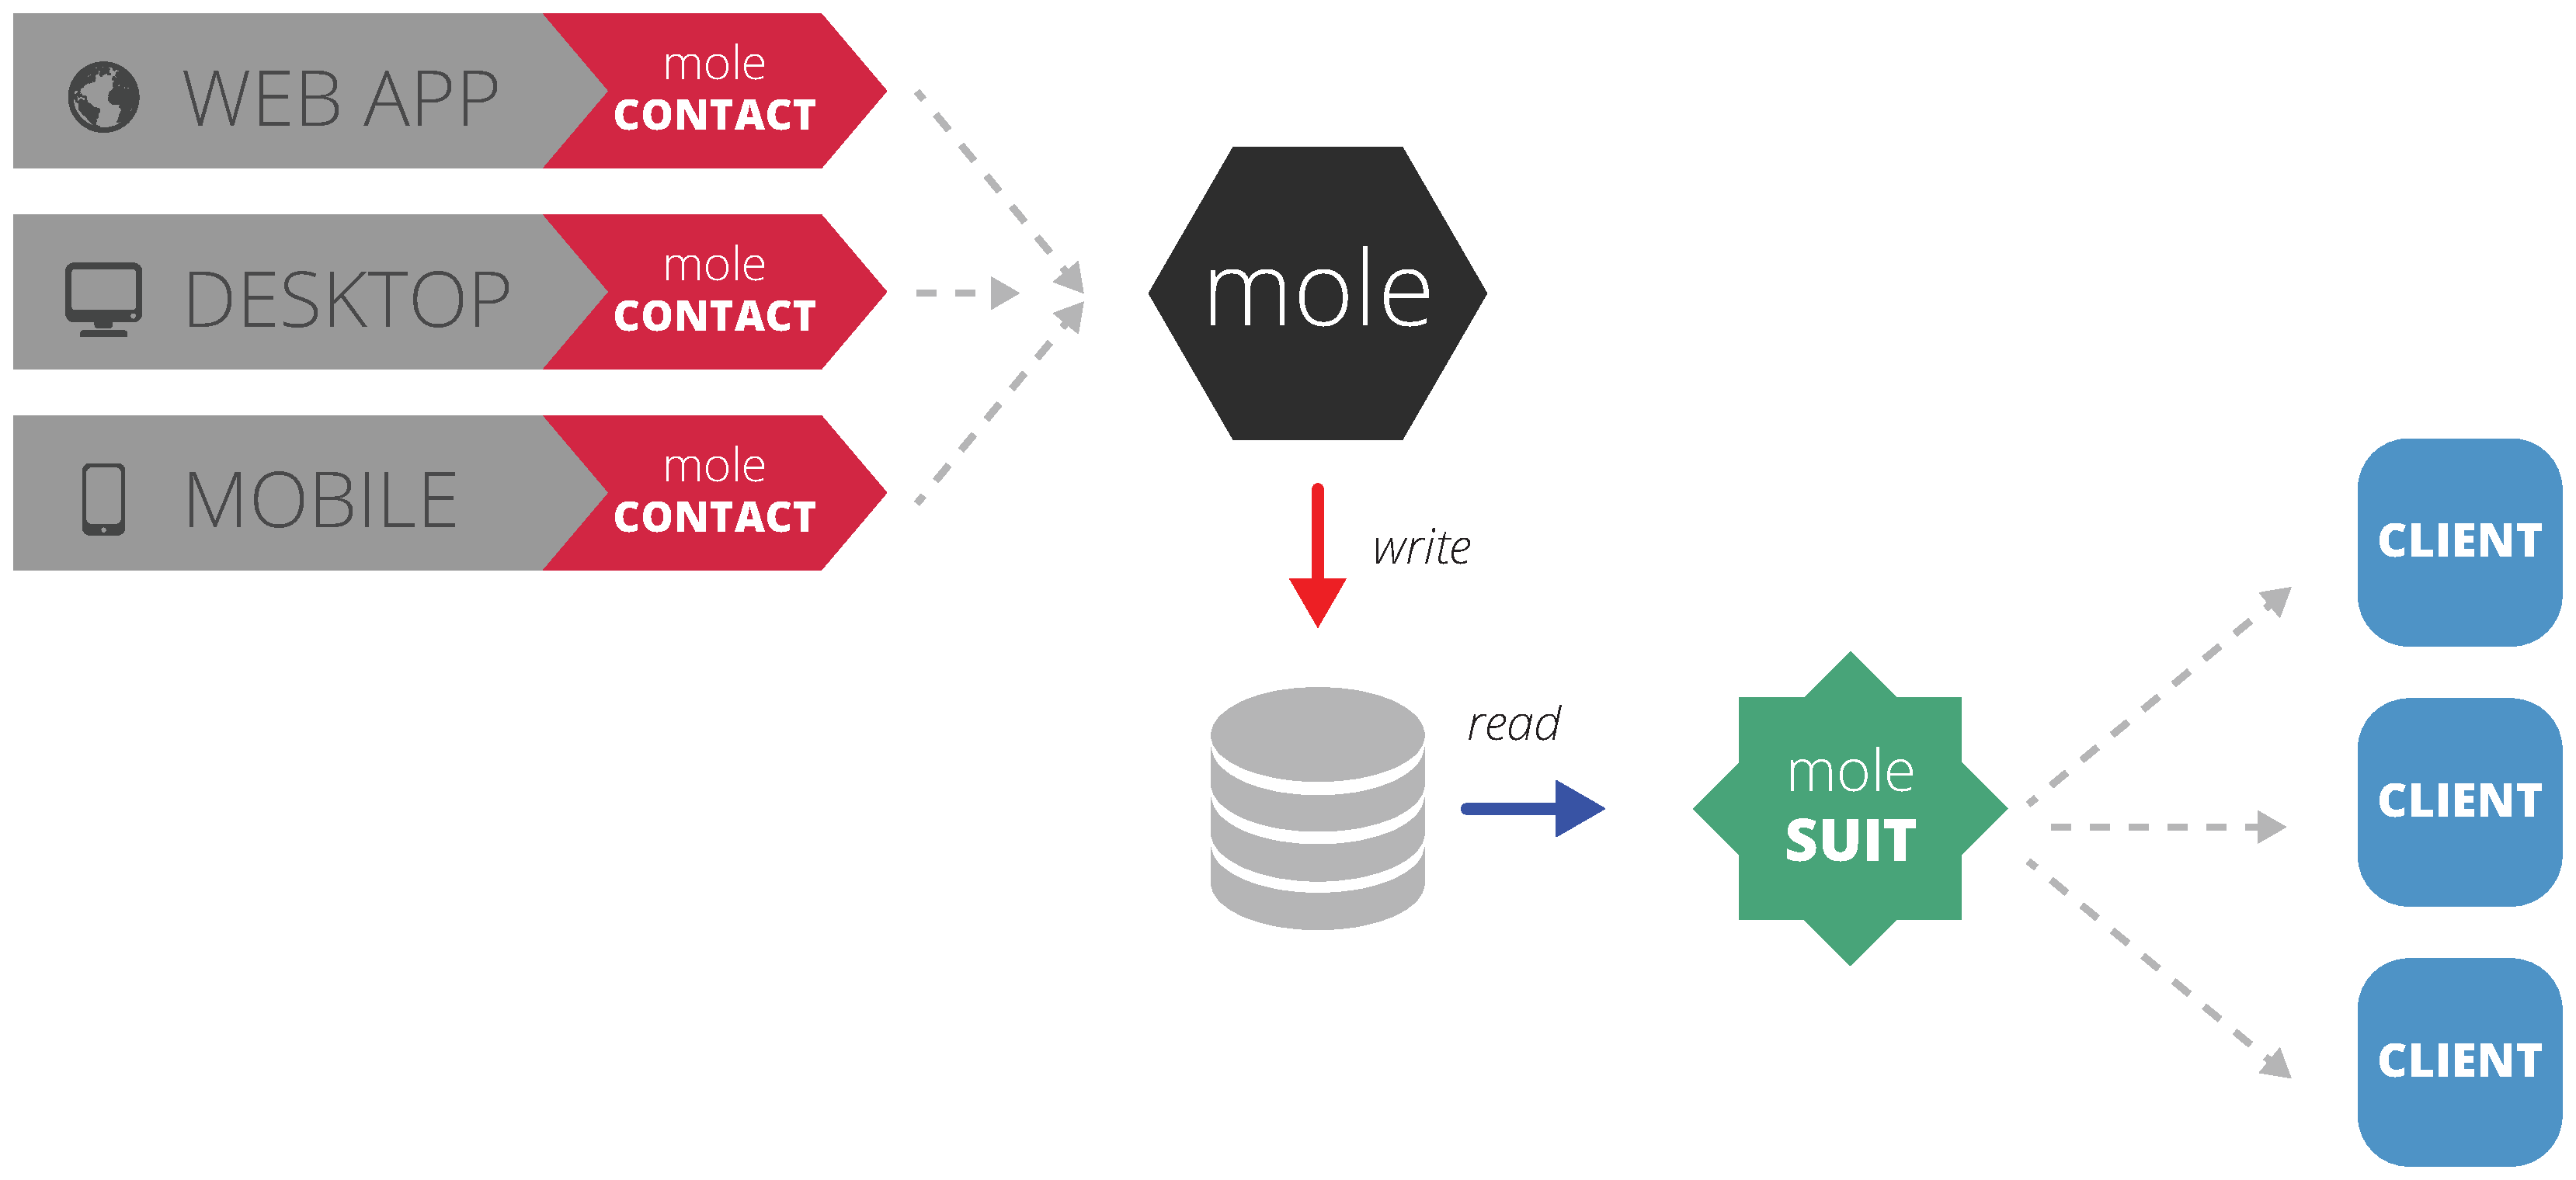
\includegraphics[width=1.0\linewidth]{./img/cqrs}
\caption[Architettura CQRS di Mole.io]{Architettura CQRS di Mole.io}
\label{fig:cqrs}
\end{figure}

i denormalizzatori possono essere aggiunti nel tempo

% estensibilit�, qui? mah...
